\documentclass[border=3pt]{standalone}
% Preâmbulo compartilhado pelos diagramas TikZ da aula 5 de IHC (Processos de Design)
\usepackage[T1]{fontenc}
\usepackage[utf8]{inputenc}
\usepackage{lmodern}
\usepackage{amsmath}
\usepackage{xcolor}
\usepackage{tikz}
\usetikzlibrary{arrows.meta,angles,quotes,decorations.pathmorphing,calc,
                positioning,shapes.geometric,shapes.misc,backgrounds,fit,
                math}

% Paleta (mesma dos SVGs originais)
% Paleta da disciplina de IHC: acento roxo (#755099), da capa do livro.
% (o nome "dblue" é mantido para não alterar todos os diagramas)
\definecolor{dblue}{HTML}{755099}
\definecolor{dorange}{HTML}{B3541E}
\definecolor{dgreen}{HTML}{4A7C59}
\definecolor{dred}{HTML}{9C4B4B}
\definecolor{dcream}{HTML}{F4F1EA}
\definecolor{dshade}{HTML}{DDD7C9}

% Função gaussiana (não normalizada por padrão de escala visual)
\pgfmathdeclarefunction{gauss}{3}{%
  \pgfmathparse{1/(#3*sqrt(2*pi))*exp(-((#1-#2)^2)/(2*#3^2))}%
}

% Estilos comuns (prefixo d... para não colidir com chaves internas do pgf)
\tikzset{
  >={Stealth[length=2mm]},
  dguide/.style={gray!55, dashed, line width=0.4pt},
  daxis/.style={gray!60, line width=0.7pt, ->},
  dbody/.style={fill=black!3, draw=black!80, line width=1pt},
  dacc/.style={draw=dblue, line width=1pt},
  dlbl/.style={black!55, font=\small},
  dsub/.style={black!45, font=\footnotesize},
  dstate/.style={circle, draw=black!80, fill=dcream, line width=1pt,
                 minimum size=17mm, font=\large, inner sep=1pt},
  dobs/.style={circle, draw=black!80, fill=dshade, line width=1pt,
               minimum size=14mm, font=\large, inner sep=1pt},
  dbox/.style={rounded corners=2pt, draw=black!80, fill=dcream, line width=1pt,
               align=center, inner sep=6pt},
  dop/.style={circle, draw=black!80, fill=white, line width=1pt,
              minimum size=6mm, inner sep=0pt, font=\small},
  dtrans/.style={->, dblue, line width=1pt},
  dmeas/.style={->, dorange, line width=1pt},
  dcurve/.style={line width=1pt, dblue},
  dcurveb/.style={line width=1.4pt, dorange},
}

\begin{document}
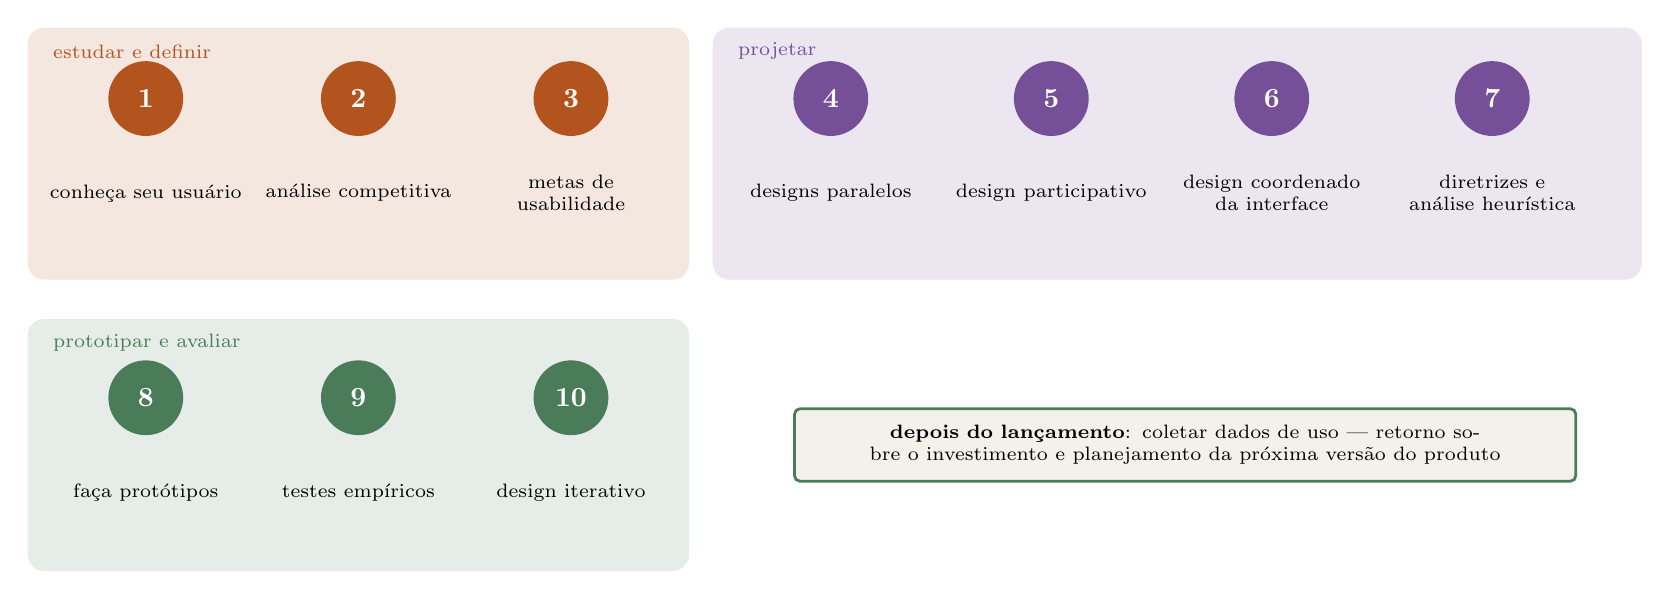
\begin{tikzpicture}[x=1cm,y=1cm,
   num/.style={circle, minimum size=0.95cm, inner sep=0pt, font=\bfseries\normalsize, text=white},
   lab/.style={text width=2.5cm, align=center, font=\scriptsize}]

  \fill[dorange!14, rounded corners=6pt] (-1.5,-1.7) rectangle (6.9,1.5);
  \fill[dblue!14, rounded corners=6pt] (7.2,-1.7) rectangle (19.0,1.5);
  \fill[dgreen!14, rounded corners=6pt] (-1.5,-5.4) rectangle (6.9,-2.2);

  \node[num, fill=dorange] at (0,0.6)   {1}; \node[lab] at (0,-0.6)   {conheça seu usuário};
  \node[num, fill=dorange] at (2.7,0.6) {2}; \node[lab] at (2.7,-0.6) {análise competitiva};
  \node[num, fill=dorange] at (5.4,0.6) {3}; \node[lab] at (5.4,-0.6) {metas de\\usabilidade};

  \node[num, fill=dblue] at (8.7,0.6)  {4}; \node[lab] at (8.7,-0.6)  {designs paralelos};
  \node[num, fill=dblue] at (11.5,0.6) {5}; \node[lab] at (11.5,-0.6) {design participativo};
  \node[num, fill=dblue] at (14.3,0.6) {6}; \node[lab] at (14.3,-0.6) {design coordenado da interface};
  \node[num, fill=dblue] at (17.1,0.6) {7}; \node[lab] at (17.1,-0.6) {diretrizes e análise heurística};

  \node[num, fill=dgreen] at (0,-3.2)   {8};  \node[lab] at (0,-4.4)   {faça protótipos};
  \node[num, fill=dgreen] at (2.7,-3.2) {9};  \node[lab] at (2.7,-4.4) {testes empíricos};
  \node[num, fill=dgreen] at (5.4,-3.2) {10}; \node[lab] at (5.4,-4.4) {design iterativo};

  \node[dbox, draw=dgreen, text width=9.5cm, font=\scriptsize] at (13.2,-3.8) {\textbf{depois do lançamento}: coletar dados de uso --- retorno sobre o investimento e planejamento da próxima versão do produto};

  \node[dlbl, font=\scriptsize, anchor=west, dorange] at (-1.3,1.2) {estudar e definir};
  \node[dlbl, font=\scriptsize, anchor=west, dblue] at (7.4,1.2) {projetar};
  \node[dlbl, font=\scriptsize, anchor=west, dgreen] at (-1.3,-2.5) {prototipar e avaliar};

\end{tikzpicture}
\end{document}
